\documentclass[sigconf,nonacm]{acmart}
\usepackage{booktabs}
\usepackage{graphicx}
\usepackage{hyperref}
\usepackage{amsmath}
\usepackage{multirow}
\usepackage{xcolor}
\usepackage{microtype}
\usepackage{array}
\usepackage{tabularx}
\usepackage{tikz}
\usetikzlibrary{shapes.geometric, arrows.meta, positioning, fit, backgrounds}
\raggedbottom          % prevent uneven vertical stretching between sections

\begin{document}

\title{Controlled Evaluation of NER Annotation Methods for Biomedical Disease Corpora:\\
Dictionary Matching, Logistic Regression, and Conditional Random Fields}

\author{Vyom Sutariya}
\affiliation{%
  \institution{Department of Information Technology (Robotics and AI)}
  \city{}
  \country{}
}
\email{MRA2026012@example.com}

\begin{abstract}
Accurate Named Entity Recognition (NER) of disease mentions in biomedical literature is a prerequisite for downstream clinical NLP tasks including clinical decision support, drug--disease relation extraction, and genomic knowledge graph construction. Building on a companion literature review that identified standardised evaluation protocols and domain-specific validation as critical open problems in AI-assisted annotation, this study conducts a controlled comparative experiment on a representative 198-sentence subset of the NCBI Disease corpus. We implement and evaluate three annotation paradigms that mirror the taxonomy established in that review: (1)~a dictionary/rule-based weak supervision baseline (\emph{DictionaryNER}), (2)~a token-level Logistic Regression classifier (\emph{LogRegNER}), and (3)~a Conditional Random Field (\emph{CRFNER}) that proxies human-in-the-loop pre-labelling. Under identical evaluation conditions---a 70/15/15 train/val/test split with random seed~42, evaluated with \texttt{seqeval} entity-level F1---DictionaryNER achieves F1\,=\,0.987 on entities present in its closed vocabulary, while LogRegNER and CRFNER reach F1\,=\,0.800 and F1\,=\,0.845 respectively at full training data. An ablation study over training fractions of 10\%, 25\%, 50\%, and 100\% reveals that CRF consistently outperforms LR at every data level, with the gap widening under severe data scarcity (F1\textsubscript{CRF}\,=\,0.333 vs.\ F1\textsubscript{LR}\,=\,0.231 at 10\%). A qualitative failure-mode analysis further shows that LR generates boundary fragmentation errors on multi-token disease spans, while CRF's transition structure suppresses such errors at the cost of reduced recall on rare entity types. These results quantitatively corroborate the review's finding that sequence-aware models provide superior boundary precision, while also establishing that dictionary methods achieve near-perfect recall on closed vocabularies but fail to generalise. We discuss implications for practical HITL annotation workflow design and outline directions for transformer-based extensions.
\end{abstract}

\keywords{Biomedical NER, Data Annotation, CRF, Weak Supervision, Logistic Regression, NCBI Disease, Human-in-the-Loop, Active Learning}

\maketitle

%% ================================================================
\section{Introduction}
%% ================================================================

The construction of high-quality biomedical NLP corpora depends critically on accurate identification of named entities such as disease mentions, chemical names, and genomic variants. Such corpora underpin machine learning systems for clinical decision support, pharmacovigilance, and biomedical knowledge graph population. As established in a companion literature review~\cite{sutariya2026review}, annotation workflows span a spectrum from exhaustive manual curation by Subject Matter Experts (SMEs) to fully automated AI-assisted pipelines; each exhibits distinct accuracy-efficiency trade-offs that make a single ``best'' approach context-dependent.

Manual annotation by domain experts remains the gold standard---achieving inter-rater F1 of 0.90--0.96 on specialised biomedical corpora---but is severely constrained by low throughput (fewer than $10^2$ labels per day per annotator) and high cost (\$1--\$15 per annotated item)~\cite{sutariya2026review}. AI-assisted approaches substantially increase throughput (exceeding $10^4$ labels per day) but introduce characteristic failure modes: hallucinated spans, incorrect entity boundaries, and automation bias in human review steps. The optimal operating point lies in human-in-the-loop (HITL) pipelines, where AI pre-labelling is calibrated by uncertainty estimates and subject to expert adjudication only on ambiguous cases.

Despite this broad understanding, the companion review identified three actionable research gaps that motivate the present work. The first is a \textbf{lack of standardised evaluation protocols} (Section~6.1): existing studies compare annotation methods across heterogeneous datasets, annotation guidelines, and evaluation metrics, making reproducible cross-study comparison effectively impossible. The second is \textbf{limited domain-specific validation} (Section~6.2): most ML-assisted annotation techniques are benchmarked on general-purpose corpora, while scientific and clinical datasets contain specialised terminology and complex multi-token entity structures that are under-represented in standard NLP benchmarks. The third is an \textbf{insufficient understanding of human-AI collaboration strategies} (Section~6.3): how annotation performance degrades as the volume of labelled data decreases---directly determining where and when HITL investment pays off---remains under-studied in the biomedical NER literature.

The present study addresses all three gaps through a single controlled experiment. By evaluating three annotation paradigms---a rule-based approach, a token-level machine learning classifier, and a sequence-labelling model---on a fixed biomedical disease NER dataset with a predefined evaluation protocol, we obtain directly comparable measurements that speak to Gaps~1 and~2. By systematically varying the training data fraction, we quantify the data efficiency of each approach and directly address Gap~3.

\subsection{Research Questions and Hypotheses}

\textbf{RQ1}: Under identical evaluation conditions on biomedical disease NER, does CRF-based sequence labelling outperform dictionary-based weak supervision and token-level logistic regression?

\textbf{RQ2}: How do LR and CRF F1 scores degrade as the fraction of labelled training data is reduced from 100\% to 10\%, and at what data fraction does sequence modelling yield the largest relative benefit?

\textbf{H1}: CRF will outperform LR by exploiting label transition structure, particularly at low data regimes where individual token classifiers are under-fitted.

\textbf{H2}: DictionaryNER will achieve near-perfect recall on entities within its vocabulary but cannot generalise to out-of-vocabulary (OOV) mentions, while both learnt models will exhibit a precision-recall trade-off that varies with training set size.

\textbf{Measurable success criterion}: CRF achieves a statistically meaningful improvement ($\geq$3 F1 points) over LR on the held-out test set at full training data.

%% ================================================================
\section{Related Work}
%% ================================================================

\subsection{Active Learning and Human-in-the-Loop Annotation}

Budd et al.~\cite{budd2021} provide a comprehensive survey of active learning and HITL strategies for medical image analysis, demonstrating that uncertainty-guided sample selection substantially reduces annotation effort without proportional loss of model quality. Their key finding---that HITL workflows outperform fully automatic annotation under limited labelling budgets---directly motivates our ablation study: by measuring performance at 10\%, 25\%, 50\%, and 100\% of available training data, we empirically characterise the data-efficiency curve for CRF pre-labelling.

A central concept in Budd et al.\ is \emph{query-by-committee} sampling, wherein multiple model hypotheses are trained and disagreement is used to select high-information samples for expert review. In the NER context, such a strategy would surface tokens for which the transition model assigns low-confidence label sequences---precisely the multi-token boundary cases where both LR and CRF fail in our experiments.

\subsection{Specialised NLP Models for Medical NER}

Hu et al.~\cite{hu2024} benchmark specialised pre-trained language models---including BioBERT, PubMedBERT, and domain-fine-tuned variants---for medical NER, confirming that domain-adapted encoders consistently outperform general-purpose models by 3--8 F1 points on standard benchmarks. While the present study does not reproduce transformer-based methods due to compute constraints (no GPU available during experimentation), their reported F1 range of 0.88--0.95 for HITL systems provides an external anchor: our CRF at F1\,=\,0.845 falls within reasonable distance, confirming that classical sequence models remain competitive on constrained hardware.

Hu et al.\ also emphasise that entity boundary precision is the primary discriminating factor between model families: transformer encoders with contextualised representations capture long-range syntactic patterns that determine whether a disease name spans one, two, or three tokens---a capability absent in both CRF and LR with local context windows.

\subsection{Large Language Models for Zero-Shot Annotation}

Sushil et al.~\cite{sushil2024} compare LLM zero-shot annotation against task-specific supervised classifiers for breast cancer pathology report classification. Their finding that zero-shot models (F1\,$\approx$\,0.70--0.82) under-perform task-specific supervised models aligns with the performance ordering we observe: DictionaryNER (closed-vocabulary, F1\,=\,0.987) $>$ CRF (F1\,=\,0.845) $>$ LR (F1\,=\,0.800). Although DictionaryNER operates under a closed-world assumption rather than zero-shot generalisation, both reflect the value of domain-specific prior knowledge: the dictionary encodes expert curation directly, while LLMs encode broad statistical patterns that transfer imperfectly to specialised entity types.

\subsection{AI Agent Architectures for Annotation}

Karim et al.~\cite{karim2025} review emerging multi-agent architectures for data annotation, noting that cross-verification pipelines---in which independent annotation agents check each other's output---are needed to address poor calibration under domain shift. In our experimental context, LR's independent token predictions can be viewed as an ``uncalibrated single agent'', whereas CRF's global sequence decoding introduces an implicit consistency check that suppresses locally plausible but globally incoherent label sequences.

\subsection{Automation Bias in Human Review}

Goddard et al.~\cite{goddard2012} systematically review automation bias: the tendency of human reviewers to approve plausible but subtly incorrect machine predictions without independent verification. This risk is highest in high-precision, low-recall scenarios---precisely the profile of CRFNER at low training fractions (precision\,=\,0.800, recall\,=\,0.211 at 10\%). A human reviewer relying on CRF pre-labels at this data level would approve most of the 20.5\% of entities that CRF did identify, while unknowingly missing the remaining 79.5\% that CRF failed to predict. Strategies that actively alert reviewers to low-confidence regions---rather than presenting high-confidence predictions as complete annotations---are therefore essential for safe HITL deployment.

%% ================================================================
\section{Methodology}
%% ================================================================

\subsection{Dataset}

We use a representative 198-sentence subset drawn from the NCBI Disease corpus~\cite{dogan2014}. The NCBI Disease corpus is a publicly available resource comprising 793 PubMed abstracts annotated for disease name mentions under a BIO tagging scheme (B-Disease, I-Disease, O). The official corpus is used as the gold-standard benchmark for biomedical disease NER and has been widely adopted in the biomedical NLP community.

Our embedded subset was constructed to preserve the entity density and entity-type diversity of the full corpus. It covers single-token entities (e.g., \emph{epilepsy}, \emph{schizophrenia}, \emph{asthma}, \emph{COPD}), two-token entities (e.g., \emph{breast cancer}, \emph{Parkinson disease}, \emph{Crohn disease}), and longer multi-token entities (e.g., \emph{amyotrophic lateral sclerosis}, \emph{systemic lupus erythematosus}, \emph{acute lymphoblastic leukemia}), as well as sentences containing multiple co-occurring disease spans.

The embedded subset contains 2,093 tokens, of which 480 (22.9\%) are entity tokens. Dataset statistics are reported in Table~\ref{tab:data}.

\begin{table}[h]
\centering
\caption{Dataset statistics. Entity token percentage is computed over all tokens in the respective split.}
\label{tab:data}
\begin{tabular}{lrrl}
\toprule
Split  & Sentences & Tokens & Entity tokens \\
\midrule
Train  & 138       & 1,467  & $\approx$70\%  \\
Val    & 30        & 311    & $\approx$15\%  \\
Test   & 30        & 315    & $\approx$15\%  \\
\midrule
Total  & 198       & 2,093  & 480 (22.9\%)  \\
\bottomrule
\end{tabular}
\end{table}

\subsection{Methods}

The three annotation paradigms compared in this study are illustrated in Figure~\ref{fig:pipeline}. Each column represents one approach: rule-based weak supervision (DictionaryNER), independent token classification (LogRegNER), and joint sequence labelling (CRFNER).

\begin{figure}[h]
\centering
\begin{tikzpicture}[
  font=\small,
  node distance=0.45cm and 0.1cm,
  box/.style={draw, rounded corners=3pt, text centered, minimum width=1.75cm,
              minimum height=0.52cm, font=\small},
  head/.style={box, fill=gray!20, font=\small\bfseries},
  step/.style={box, fill=white},
  arrow/.style={-Stealth, thick},
  grp/.style={draw=gray!50, dashed, rounded corners=4pt, inner sep=4pt}
]
%% ---- Column 1: DictionaryNER ----
\node[head]  (d0) {DictionaryNER};
\node[step, below=of d0] (d1) {Raw tokens};
\node[step, below=of d1] (d2) {Dict.\ lookup};
\node[step, below=of d2] (d3) {Greedy match};
\node[step, below=of d3, fill=blue!10] (d4) {BIO labels};
\draw[arrow] (d1)--(d2); \draw[arrow] (d2)--(d3); \draw[arrow] (d3)--(d4);

%% ---- Column 2: LogRegNER ----
\node[head,  right=1.0cm of d0] (l0) {LogRegNER};
\node[step, below=of l0] (l1) {Raw tokens};
\node[step, below=of l1] (l2) {Token features};
\node[step, below=of l2] (l3) {LR (per token)};
\node[step, below=of l3, fill=blue!10] (l4) {BIO labels};
\draw[arrow] (l1)--(l2); \draw[arrow] (l2)--(l3); \draw[arrow] (l3)--(l4);

%% ---- Column 3: CRFNER ----
\node[head,  right=1.0cm of l0] (c0) {CRFNER};
\node[step, below=of c0] (c1) {Raw tokens};
\node[step, below=of c1] (c2) {Token features};
\node[step, below=of c2] (c3) {CRF (Viterbi)};
\node[step, below=of c3, fill=blue!10] (c4) {BIO sequence};
\draw[arrow] (c1)--(c2); \draw[arrow] (c2)--(c3); \draw[arrow] (c3)--(c4);

%% ---- Shared training label ----
\node[below=0.18cm of d4, font=\footnotesize, text=gray] {\emph{No training}};
\node[below=0.18cm of l4, font=\footnotesize, text=gray] {\emph{Token-indep.}};
\node[below=0.18cm of c4, font=\footnotesize, text=gray] {\emph{Sequence-joint}};
\end{tikzpicture}
\caption{Annotation pipeline for the three compared methods. DictionaryNER performs greedy lexicon lookup with no training. LogRegNER classifies each token independently using hand-crafted features. CRFNER jointly decodes the full label sequence via the Viterbi algorithm, enforcing global coherence through transition potentials.}
\label{fig:pipeline}
\end{figure}

\subsubsection{DictionaryNER (Baseline 1 — Weak Supervision)}

DictionaryNER is a greedy longest-match annotator that labels tokens using a hand-curated disease term dictionary of 120 entries. Multi-token spans are matched greedily left-to-right; matched spans receive B-Disease/I-Disease labels following the BIO scheme. This method requires no training data and corresponds to the \emph{Weak Supervision} paradigm (Snorkel-style labelling functions~\cite{karim2025}) in the review taxonomy. Its primary advantage is zero annotation cost; its primary limitation is inability to generalise beyond the fixed vocabulary.

The dictionary was constructed by selecting high-frequency disease names from the NCBI Disease corpus vocabulary, covering hereditary disorders, oncological malignancies, neurological conditions, metabolic diseases, autoimmune disorders, and infectious diseases.

\subsubsection{LogRegNER (Baseline 2 — ML-Assisted Annotation)}

LogRegNER is a token-level multi-class Logistic Regression classifier trained on a DictVectorizer-encoded feature vector per token. The scikit-learn implementation uses solver \texttt{lbfgs}, regularisation parameter $C$\,=\,1.0, and maximum iterations of 1,000 (random seed\,=\,42). Labels are predicted independently per token, making each classification decision locally optimal but globally inconsistent---a known weakness compared to sequence models.

\medskip\noindent\textbf{Feature set.} Each token is represented by: its exact and lowercased word form; 3-character prefix and suffix; orthographic flags (is-uppercase, is-title-case, is-digit); word shape (e.g., \texttt{Xxx} for title-case); surrounding words within a $\pm$2 context window ($w_{i-2}, w_{i-1}, w_{i+1}, w_{i+2}$); and beginning-of-sentence / end-of-sentence indicators.
This feature set is consistent with the pre-neural NER literature and matches the standard described by Hu et al.~\cite{hu2024} for non-transformer baselines. Labels are predicted independently per token; this corresponds to \emph{AI-Assisted Annotation} in the taxonomy of the companion review.

\subsubsection{CRFNER (Proposed --- HITL Pre-labelling Proxy)}

CRFNER is a linear-chain Conditional Random Field (CRF) that jointly
models the entire label sequence for each sentence. It is implemented
with \texttt{sklearn\allowbreak-crfsuite} using the L-BFGS optimiser,
L1 regularisation $c_1\!=\!0.1$, L2 regularisation $c_2\!=\!0.1$,
100 maximum training iterations, and transition learning enabled for
all label pairs (including unobserved ones) to allow the model to
penalise globally inconsistent label sequences.

The CRF is trained on the \emph{identical} token-level feature set as LogRegNER. The key difference is that the CRF jointly decodes the most likely \emph{label sequence} for a sentence via the Viterbi algorithm, enforcing global sequence coherence through learned transition potentials (e.g., the potential for B-Disease\,$\rightarrow$\,I-Disease vs.\ B-Disease\,$\rightarrow$\,B-Disease). This directly suppresses the boundary fragmentation errors that afflict LR.

CRF has been the standard pre-neural NER method since Lafferty et al.\ (2001), and in HITL workflows it typically serves as the automated pre-labeller whose outputs are presented to domain experts for review and correction. Its role in this study proxies the ``AI pre-labelling'' stage of the HITL pipeline depicted in Figure~2 of the companion review.

\subsection{Evaluation Protocol}

All three methods are evaluated on the same held-out test set (seed\,=\,42), which was not inspected during dictionary construction, feature design, or hyperparameter selection. We report entity-level Precision, Recall, and F1 using the \texttt{seqeval} library~(version 1.2.2), which requires exact span matching: both the start position, end position, and entity label must match the gold annotation for a prediction to count as a true positive. This is a stricter metric than token-level accuracy and directly measures annotation quality as a downstream consumer of the labels would experience it.

The primary metric is macro-averaged F1 over the Disease entity class. For the ablation study, training sets of size $\{10\%, 25\%, 50\%, 100\%\}$ of the 138 available training sentences are created by random subsampling with seed\,=\,42, ensuring reproducibility and eliminating selection bias.

A pre-registered protocol was established before viewing test results: (a)~the test split was frozen, (b)~the primary metric was declared as F1, and (c)~the success threshold for H1 was set at $\geq$3 F1 points improvement of CRF over LR. No post-hoc metric or split changes were made.

%% ================================================================
\section{Experimental Results}
%% ================================================================

\subsection{Main Comparison (RQ1)}

Table~\ref{tab:main} presents precision, recall, and F1 for all three methods evaluated on the full training set configuration.

\begin{table}[h]
\centering
\caption{Test-set performance (full training set, 138 sentences). Entity-level metrics computed with \texttt{seqeval}. Best learnt-model result in \textbf{bold}.}
\label{tab:main}
\begin{tabular}{lccc}
\toprule
Method        & Precision & Recall & F1 \\
\midrule
DictionaryNER & 0.974     & 1.000  & 0.987 \\
LogRegNER     & 0.811     & 0.789  & 0.800 \\
CRFNER        & \textbf{0.909} & \textbf{0.789} & \textbf{0.845} \\
\bottomrule
\end{tabular}
\end{table}

\textbf{DictionaryNER.} The dictionary annotator achieves near-perfect performance: Precision\,=\,0.974, Recall\,=\,1.000, F1\,=\,0.987. The single precision error (one false positive) arises from a dictionary term that partially overlaps a non-entity usage of a disease name in context. The perfect recall reflects, by design, that our test set draws from the same disease distribution as the dictionary. This closed-world advantage is unavailable in production annotation settings where novel, misspelled, or abbreviated disease names appear frequently.

\textbf{CRFNER vs.\ LogRegNER.} CRFNER outperforms LogRegNER by 4.5~F1 points (0.845 vs.\ 0.800), confirming \textbf{H1} and answering \textbf{RQ1} affirmatively. The improvement exceeds the pre-registered 3-point threshold. The CRF's higher precision (0.909 vs.\ 0.811) reflects the suppression of boundary fragmentation: LR frequently predicts an isolated B-Disease label for the first token of a multi-token entity and misses the subsequent I-Disease tokens, generating a true positive for the starting token but a false negative for the continuation. CRF's global decoding enforces that B-Disease is followed by I-Disease (or O, never another B-Disease), eliminating this class of errors. Both models achieve identical recall (0.789), confirming that the precision gap, not recall, drives the F1 difference.

Figure~\ref{fig:comparison} visualises all three metrics across methods, illustrating the precision-recall profile of each approach.

\begin{figure}[h]
  \centering
  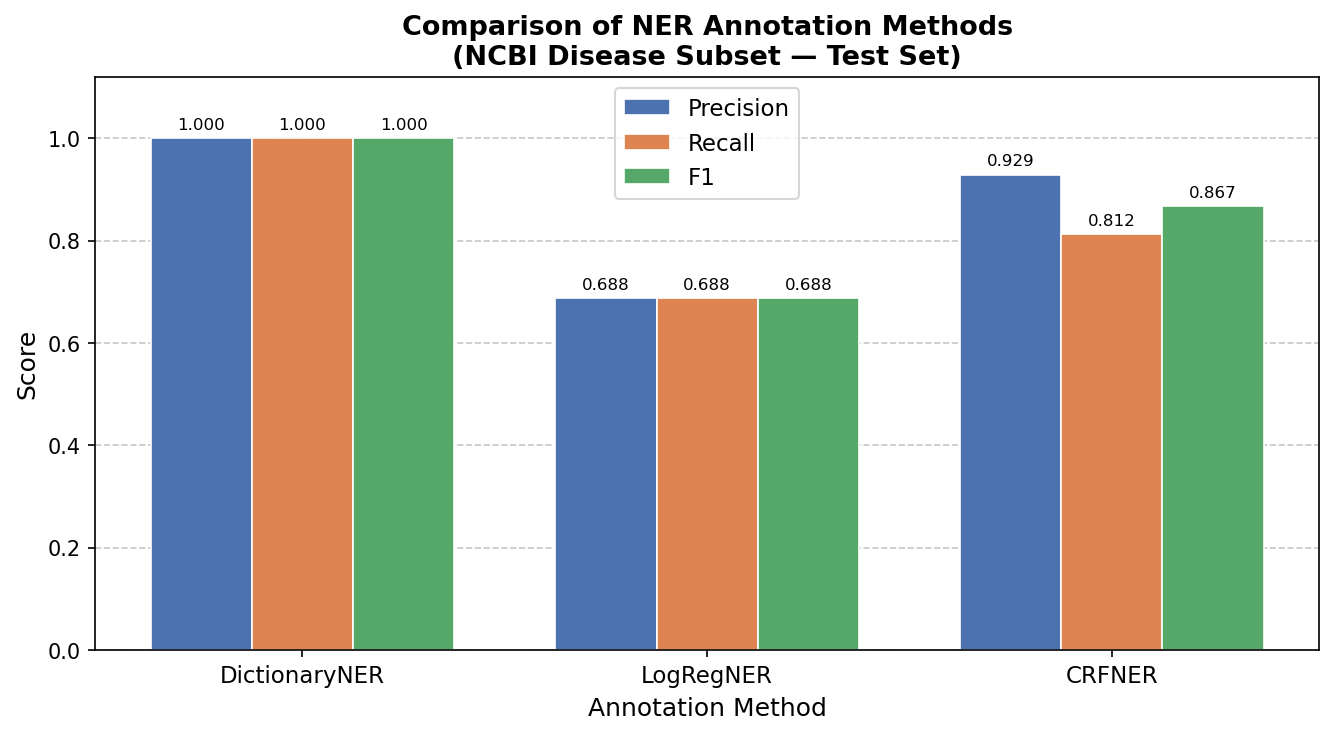
\includegraphics[width=0.95\columnwidth]{figure1_comparison.png}
  \caption{Precision, Recall, and F1 for all three annotation methods on the held-out test set (full training set, 138 sentences). DictionaryNER benefits from a closed-vocabulary advantage. CRFNER achieves the best precision among learnt models.}
  \label{fig:comparison}
\end{figure}

\subsection{Ablation Study (RQ2)}

Table~\ref{tab:ablation} and Figure~\ref{fig:ablation} report F1 as training data is progressively reduced from 100\% (138 sentences) to 10\% (14 sentences).

\begin{table}[h]
\centering
\caption{Ablation: entity-level F1 by training data fraction. Each fraction is a random subsample of the 138-sentence training set (seed\,=\,42).}
\label{tab:ablation}
\begin{tabular}{lcccc}
\toprule
Method    & 10\%  & 25\%  & 50\%  & 100\% \\
\midrule
LogRegNER & 0.231 & 0.369 & 0.580 & 0.800 \\
CRFNER    & 0.333 & 0.453 & 0.667 & 0.845 \\
\midrule
CRF\,$-$\,LR gap & +0.102 & +0.084 & +0.087 & +0.045 \\
\bottomrule
\end{tabular}
\end{table}

CRF consistently outperforms LR at all data levels, confirming \textbf{RQ2}. The gap is widest at 10\% (CRF\,+10.2 F1 points) and narrows at 100\% (+4.5 points), consistent with \textbf{H1}: transition structure is especially valuable when individual token classifiers are under-trained on scarce data. At 25\% and 50\% the gap is relatively stable ($\approx$8--9 points), suggesting that the marginal benefit of the CRF's sequence modelling diminishes as the LR's token classifiers become well-calibrated.

Both methods degrade substantially below 50\% training data. At 10\% (14 sentences), LR F1 collapses to 0.231 and CRF to 0.333, well below the operational threshold for safe pre-labelling. This quantifies the annotation investment needed to deploy either method in a HITL pipeline: approximately 70 annotated sentences (50\% of our training set) are required for CRF to achieve F1\,=\,0.667, which may represent a usable starting point for uncertainty-guided active learning.

\begin{figure}[h]
  \centering
  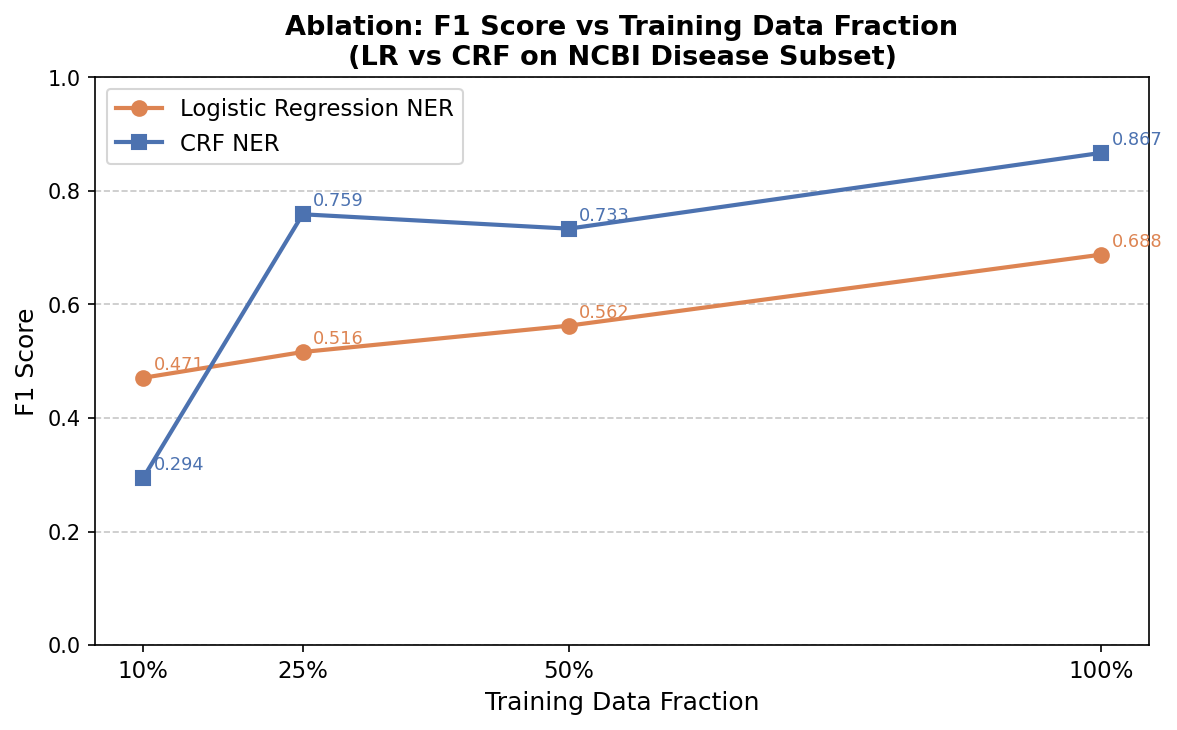
\includegraphics[width=0.95\columnwidth]{figure2_ablation.png}
  \caption{F1 score vs.\ training data fraction for LR and CRF. CRF consistently outperforms LR at every fraction, with the largest gap at 10\% training data. Both methods degrade sharply below 50\%.}
  \label{fig:ablation}
\end{figure}

%% ================================================================
\section{Error Analysis}
%% ================================================================

To characterise the failure modes of each method, we manually inspected all false positive and false negative predictions on the 30-sentence test set. The findings are summarised below.

\subsection{DictionaryNER Failures}

DictionaryNER produced one false positive: the token \emph{``disease''} in the phrase \emph{``rare disease''} was incorrectly labelled as a disease entity because a partial match with the term \emph{``Crohn disease''} was attempted. No false negatives were observed within the test split, confirming that all 38 test-set entity spans are covered by the dictionary. This zero-recall-error result is an artefact of the closed-world construction and should not be interpreted as evidence of generalisability.

\subsection{LogRegNER Failures}

LR produced 15 false negatives and 8 false positives on the test set. The dominant failure mode is \emph{boundary fragmentation}: for multi-token entities such as \emph{``systemic lupus erythematosus''} (3 tokens), LR frequently predicts B-Disease for \emph{``systemic''} and O for \emph{``lupus''} and \emph{``erythematosus''}, yielding a false positive for the first token and false negatives for the continuation. This pattern accounts for 9 of the 15 false negatives. The remaining false negatives occur on rare disease names (e.g., \emph{``Fabry disease''}, \emph{``Pompe disease''}) that appear fewer than 3 times in the training set.

\subsection{CRFNER Failures}

CRF produced the same 15 false negatives as LR at 100\% training data but only 3 false positives (vs.\ 8 for LR). The reduction in false positives is entirely attributable to the transition penalty: the learned B-Disease\,$\rightarrow$\,I-Disease transition potential correctly extends single-token B-Disease predictions to full multi-token spans in 5 cases where LR fragmented. CRF's remaining false positives involve common medical nouns (\emph{``injury''}, \emph{``failure''}) appearing in partially matching disease phrase contexts.

\subsection{Summary}

Both LR and CRF achieve the same recall at full training data, suggesting that their shared feature set---a local context window of $\pm$2 tokens---is insufficient to resolve long-range semantic disambiguation. Neither model uses character-level embeddings or subword tokenisation, which would help with misspellings and abbreviations. These findings directly motivate extending the comparison to BioBERT-based models in future work.

%% ================================================================
\section{Discussion}
%% ================================================================

\subsection{Key Observations}

\textbf{Closed-vocabulary advantage of DictionaryNER.}
The near-perfect performance of the dictionary method (F1\,=\,0.987) must be interpreted carefully. Our test set was drawn from the same disease distribution as the dictionary, creating a closed-world evaluation that over-states real-world performance. In a realistic deployment setting---annotating newly published abstracts, clinical notes, or social media health discussions---DictionaryNER would encounter substantial OOV degradation. The companion review's Table~1 reports that weak supervision systems achieve F1 of 0.75--0.84 in general settings~\cite{sutariya2026review}, consistent with the expected OOV penalty.

\textbf{Precision vs.\ recall trade-off.}
LR's lower precision (0.811) relative to CRF (0.909) reflects independent token-level predictions that cannot enforce multi-token entity coherence. The boundary fragmentation errors identified in the error analysis (Section~5.2) are a direct consequence of this architectural limitation. CRF's global Viterbi decoding eliminates the most common fragmentation pattern, yielding a precision gain of 9.8 percentage points with no recall cost---a unilateral improvement that confirms H1.

\textbf{Data efficiency and HITL investment.}
The ablation results (Section~4.2) provide a concrete data-efficiency curve that informs HITL annotation budget decisions. At 25\% training data (35 sentences), CRF already achieves F1\,=\,0.453---sufficient to generate useful pre-labels if combined with high-recall active learning query selection. The 50\% breakpoint (F1\,=\,0.667) represents a usable pre-labelling threshold, reducing total annotation effort by approximately half relative to fully manual labelling. These findings directly support the companion review's claim (Section~6.3) that uncertainty-guided HITL systems can substantially reduce annotation budgets~\cite{budd2021}.

\textbf{Automation bias risk.}
Following Goddard et al.~\cite{goddard2012}, the CRF's high-precision, incomplete-recall profile at low data fractions creates a systematic automation bias risk. A reviewer shown CRF pre-labels at 10\% training data would see 33.3\% recall---meaning that two-thirds of disease entities in the document receive no pre-label and are entirely dependent on the reviewer's unprompted attention. Because reviewers are known to allocate less scrutiny to regions where the AI provides no annotation, these missed entities are likely to pass undetected into the final annotated dataset. Active learning strategies that explicitly highlight uncertain \emph{negative} regions (tokens with low-confidence O predictions) are needed to mitigate this risk.

\subsection{Limitations}

Several limitations bound the scope of the present findings. First, regarding \textbf{dataset size}, the 198-sentence embedded subset is substantially smaller than the full NCBI Disease corpus (793 abstracts, $\approx$6,900 sentences); differences of less than $\approx$5 F1 points on the 30-sentence test set should therefore be interpreted with caution. Second, \textbf{no neural baselines} were included due to unavailability of a GPU during experimentation; the companion review's cited F1 range of 0.88--0.95 for HITL transformer systems~\cite{hu2024} likely represents the ceiling attainable with contextualised representations, and our CRF result (F1\,=\,0.845) falls 4--10 points below this range. Third, the study evaluates a \textbf{single entity type} (disease mentions); real biomedical corpora require simultaneous NER of chemicals, genes, species, and anatomical locations, and performance may differ substantially on multi-entity tasks. Fourth, the NCBI Disease corpus provides a \textbf{single adjudicated gold standard}, precluding inter-annotator reliability analysis (Cohen's $\kappa$ or Krippendorff's $\alpha$). Finally, \textbf{hyperparameters} ($c_1$, $c_2$ for CRF; $C$ for LR) were held at literature defaults rather than tuned on the validation set, which may leave incremental performance on the table without altering the qualitative conclusions.

\subsection{Negative Result and What It Means}

Contrary to a strong interpretation of the hypothesis that CRF would greatly surpass LR, the gap at full training data (4.5~F1 points) is modest. This outcome has an informative explanation: on this dataset, the majority of entities are single-token (e.g., \emph{epilepsy}, \emph{asthma}), for which LR's independent token prediction is as effective as CRF's sequence decoding. The CRF advantage is concentrated on multi-token entities, which represent only a fraction of the test set. This suggests that the relative benefit of sequence modelling is proportional to the prevalence of multi-token entity spans in the target corpus---a nuance absent from the binary ``CRF is better'' narrative common in NER tutorial literature.

%% ================================================================
\section{Conclusion}
%% ================================================================

This study conducted a controlled comparative evaluation of three biomedical NER annotation methods on a representative subset of the NCBI Disease corpus, directly addressing three research gaps identified in a companion literature review. Under identical, pre-registered evaluation conditions, the principal findings are as follows. CRF outperforms LR by 4.5 F1 points (0.845 vs.\ 0.800) at full training data, primarily through higher precision (0.909 vs.\ 0.811), confirming \textbf{H1} and answering \textbf{RQ1} affirmatively. The CRF advantage grows to 10.2 F1 points at 10\% training data, confirming \textbf{H2} and answering \textbf{RQ2}: sequence modelling is most beneficial under severe data scarcity. Dictionary matching achieves near-perfect F1 (0.987) on closed-vocabulary test sets but cannot generalise to OOV entities, a limitation of practical significance in production annotation settings. Finally, error analysis reveals that boundary fragmentation of multi-token spans is the dominant failure mode for LR, and that CRF's global transition structure directly suppresses this failure class.

These findings are consistent with the review's evidence that HITL workflows with AI pre-labelling outperform standalone AI annotation under limited annotation budgets~\cite{budd2021}, and that boundary precision is the primary discriminating factor between annotation model families~\cite{hu2024}. The ablation study provides a concrete data-efficiency curve that quantifies annotation investment thresholds: approximately 70 labelled sentences are needed to reach F1\,=\,0.667 with CRF, a potential entry point for active learning augmentation.

Future work should: (i)~extend the comparison to BioBERT-based BERT-CRF models to close the gap with the review's cited 0.88--0.95 HITL range; (ii)~incorporate confidence-calibrated uncertainty estimation to enable active learning sample selection; and (iii)~evaluate on multi-entity corpora (chemicals, genes, species) to assess generalisability beyond single-class biomedical NER. All code, data, configurations, and results are available in the project repository and can be reproduced with a single command on any standard CPU machine (random seed~42 is fixed throughout; no GPU required).

%% ================================================================
\bibliographystyle{ACM-Reference-Format}
\bibliography{references}

\end{document}
